\sectionSrc{Instruction format validation}
{parser\_library/src/context/instruction.h,parser\_library/src/checking/operand.h,parser\_library/src/checking/instr\_operand.h}

\label{checker}
One of the essential ways to provide results of the parsing to the user is through error messages. Many of these messages are created in \emph{Instruction checker} which validates the usage of different kinds of instructions.

Instruction checker is an abstract class for various types of instructions. Its \TT{check} method is being called from the instruction processors~\ref{chap:process} to check whether the specific instruction is used with correct parameters. As assembler and machine instructions have different formats, we derive separate \emph{assembler} and \emph{machine} checkers from the instruction checker. CA instructions do not have a derived checker class as they are all being checked during their interpretation.

The checkers need an access to the definitions of all possible instructions. These instructions are stored statically inside an object called \emph{instruction}. It consists of 4 different containers:
\begin{itemize}
	\item \emph{machine\_instructions} is a map of instruction names to machine instruction object, which contains various data such as format, size or vector of instruction's operands.
	\item \emph{mnemonic\_codes} maps instruction names to their mnemonic code. The mnemonic codes are simplified versions of specific machine instructions, substituting one of the operands by a default value. The mnemonic code objects provides a list of operands to be substituted along with the original instruction name.
	\item \emph{assembler\_instructions} is similar to the machine instructions. However, as the assembler instructions do not have formats, these classes only state minimum/maximum number of operands for specific instruction.~In~\cref{sub:asm_check}, we explain how the assembler instructions are validated.
	\item \emph{ca\_instructions} only contains a list of possible CA instructions.
\end{itemize}

Both assembler and machine checker works in a similar manner:
\begin{enumerate}
	\item Either assembler or machine processor calls the \TT{check} method of its respective checker. This method accepts the instruction name, the vector of used operands, the range of statement and the diagnostic collector.
	\item Checker finds the correct instruction based on the provided name and calls the \TT{check} method of its instruction class, along with the same parameters as mentioned above.
	\item The instruction itself compares its possible operands with the used operands.
	\item More validations may be necessary, based on the instruction.
	\item In case of mismatch, a diagnostic is added to the passed diagnostic container.
\end{enumerate}

\subsectionSrc{Machine instruction checker}
{parser\_library/src/checking/instruction\_checker.h,parser\_library/src/context/instruction.h}

All machine instructions have a precisely defined format which makes the validation based on these formats straightforward. Machine instructions checker operates with machine instructions and their mnemonic codes.

The formats are defined by several basic operands such as register or address and state which combination of these operands are acceptable. For example, instruction LR has format RR, which means it accepts only 2 arbitrary (but correct) registers. 

\begin{figure}
	\centering
	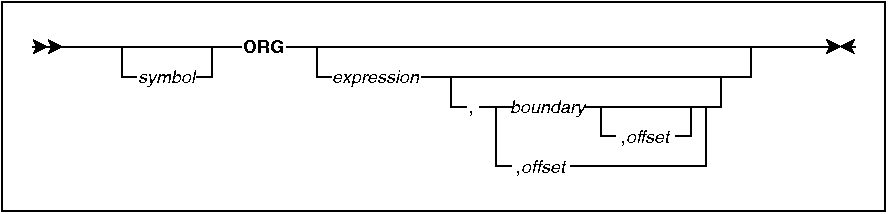
\includegraphics[width=\textwidth]{img/org_diagram}
	\caption{Operand diagram for the ORG instruction.}
	
	\label{fig01:check}
\end{figure}

\subsectionSrc{Assembler instruction checker}
{parser\_library/src/checking/asm\_instr\_class.h,parser\_library/src/checking/asm\_instr\_check.h}
\label{sub:asm_check}

Validation of assembler instructions is more complicated as there are no pre-defined formats for them. Each of them is described by custom operand diagrams, which demonstrate the dependencies and relations between operands of a specific instruction. An example of such diagram for the ORG instruction is shown in \cref{fig01:check}. As an addition to the basic operands used for machine instructions, each assembler instruction might have its own operands, called keywords.

Due to these irregularities, we derive instruction-specific classes from assembler instruction class. Each of them implements the \TT{check} method, to provide the customized checking.

\subsubsectionSrc[0.55\linewidth]{Data Definition checking}
{parser\_library/src/checking/data\_definition/data\_def\_fields.h,parser\_library/src/checking/data\_definition/data\_def\_type\_base.h,parser\_library/src/checking/data\_definition/data\_def\_types.h,parser\_library/src/checking/data\_definition/data\_definition\_operand.h}

Data definition is a type of operand in HLASM. It represents data that is assembled directly into object code (see \cref{asm_instrs}).

Since there are many types of data definition, there is a data definition subcomponent of instruction validation. Whenever any component of the project needs information about a data definition operand, it can use this subcomponent. It analyzes each type of data definition and is able to return its length, attributes and check its validity.

Each type is different and many have special conditions that must be met to be valid. That is why there is an abstract class \TT{data\_def\_type\_base}, which has 38 implementations --- one for each type (including type extensions). The types are then available in a static associative map that maps names of types to their representations.

